\section{Linear Regression with one variable}
  Regression being a part of Supervised Learning is used for estimating data (real-valued output).  

  \subsection{Cost Function}
    This function measures the performance of a Machine Learning model for given data.

    \textbf{Hypothesis}: $ h_ \theta(x) = \theta_0 + \theta_1x $

    \textbf{Parameters:} $ \theta_0, \theta_1 $

    \textbf{Cost Function:} 
    \begin{equation} \label {eq:1}
      J( \theta_0, \theta_1 ) = 1/2m \sum_{i=1}^{m} (h_\theta(x^{(i)})-y^{(i)})^2 
    \end{equation} 

    \textbf{Goal:} Minimize cost function with $ \theta_0, \theta_1 $ as parameters.

  \subsection{Gradient Descent}

    \textbf{Basic idea:}
    \begin{itemize}
    \item Start with some $ \theta_0, \theta_1 $
    \item Keep changing $ \theta_0, \theta_1 $ to reduce $ J(\theta_0, \theta_1) $ until we end up at minima.
    \end{itemize} 

    \textbf{Algorithm:}
     repeat until convergence:
    \begin{equation} \label {eq:2}
      \theta_j := \theta_j - \alpha \frac{\partial {J(\theta_0, \theta_1)}}{\partial \theta_j}
    \end{equation} 

    (for  $j = 0, 1 $  ,here).  

    \textbf{Intuition:} 
    If $\alpha$ is too small, the descent can be slow and if too large, descent may fail to converge or even diverge.
    Gradient descent can converge to a local minimum, even with a fixed learning rate $\alpha$. As we approach local minimum, gradient descent will automatically take smaller steps. So, no need to decrease $\alpha$ over time. 

  \subsection{Gradient Descent for linear regression}
    Combining gradient descent algorithm with linear regression model, we get:

    \begin{equation} \label {eq:3}
      j = 0 : \frac{\partial {J(\theta_0, \theta_1)}}{\partial \theta_0} = 1/2 \sum_{i=1}^{m} (h_\theta(x^{(i)})-y^{(i)}) 
    \end{equation}

    \begin{equation} \label {eq:4}
      j = 1 : \frac{\partial {J(\theta_0, \theta_1)}}{\partial \theta_1} = 1/2 \sum_{i=1}^{m} (h_\theta(x^{(i)})-y^{(i)}).x^{(i)}
    \end{equation}

    Now, we can repeat \ref{eq:3} and \ref{eq:4} until convergence to obtain the minima.

    "Batch" gradient descent: Each step of gradient descent uses all the training examples.
    For eq. "m" batches in equation \ref{eq:1}.

\section{Multivariate Linear Regression}
  Linear regression involving more than one variable. For eq., Predicting the price of a house based on parameters "Plot Area", "No. of Floors", "Connectivity with markets", etc.

  \subsection{Multiple Features}
    The multivariable form of the hypothesis is as follows:
    \begin{equation} \label {eq:5}
      h_\theta(x) = \theta_0 + \theta_1x_1 + \theta_2x_2 + \theta_ 3x_3 + ... + \theta_{n}x_n.  
    \end{equation}
    This hypothesis function can be concisely represented as:
    \begin{equation}
      h_\theta(x) = \theta^{T}x
    \end{equation}
    where $ \theta^T $ is a 1xn matrix consisting of $ \theta_0, \theta_1, \theta_2 ... \theta_n $.


  \subsection{Gradient Descent for Multiple Variables}
    Gradient descent formula for Multiple variables will be similar to that of a single variable.

    \begin{equation} \label {eq: GD for multiple}
      \theta_j =  \theta_j - \alpha \frac{1}{m} \sum_{i=1}^{m} (h_\theta(x^{(i)})-y^{(i)}).x_j^{(i)}
    \end{equation}

    Repeating this equation until convergence will give the minima. \footnote[1]{$x_0 = 1$ in equation \ref{eq: GD for multiple}}

  \subsubsection{Feature Scaling}
    Feature Scaling is used to reduce the number of iterations in Gradient Descent. The basic idea of feature scaling is to bring all the features on the same scale. (in general, we try to approximate every feature in the range $ -1 < x_i < 1 $)
    \\ \\ Reducing the number of iteration doesn't mean making computation of each step easier. And also it does not affect the computational efficiency of Normal Equation.

  \subsubsection{Mean Normalisation}
    Mean Normalisation makes features to have approximately zero mean.

  \subsubsection{Learning Rate}
    If $\alpha$ is too small: slow convergence.

    if $\alpha$ is too large: $J(\theta)$ may not decrease on every iteration, or may not converge.

  \subsubsection{Polynomial Regression}
    Selecting proper polynomial for fitting data is very important.

    \begin{figure}[h]
      \centering
      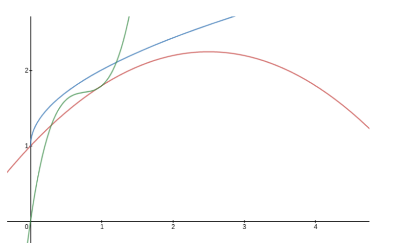
\includegraphics[width=8cm, height=5cm]{polyreg.png}
    \end{figure}

    \textbf{Red:} Quadratic

    \textbf {Blue:} Square root funtion $ \theta_0+\theta_1x+\theta_2\sqrt{x} $

    \textbf {Green:} Cubic function

\section{Normal equation}
  Normal Equation is a method to solve for $\theta_T$ analytically, by creating a $m\times(n+1)$ matrix $X$ and another $m\times1$ matrix $Y$.\footnote[2]{Every element of the first column of matrix $X$ is 1 and other are the feature's coefficient}

  Mathematically $\theta$ is given as:
  \begin{equation} \label {eq: theta}
    \theta = (X^TX)^{-1}X^ty
  \end{equation}

  \begin{tabular}{ |c|c|}
    \hline
    \textbf{Gradient Descent} & \textbf{Normal Equation} \\
    \hline
    Need to choose $\alpha$ & No need to choose $\alpha$ \\
    Needs many iterations & Don't need to iterate \\
    Works well with large n & Slow for large n \\
    \hline
  \end{tabular}

  \vspace{5mm}

  \subsubsection{Reasons for non-invertibility of $X^T X$}
    \begin{itemize}
      \item Redundant features (linear dependence) \footnote[3]{Eg. Using both $m^2 \  \& \  (feet)^2$ features}
      \item Too many features (m $<=$ n) 
    \end{itemize}
  
  % \lstinputlisting[language=Octave, caption=Octave Implementation for Linear Regression Algorithms]{linearRegression.m}
